\documentclass{beamer}
\usepackage{graphicx}
\usepackage{paralist}
\usepackage{outlines}

\title{Color Sampling Tools}
\author{Mendocino College - Digital Image Manipulation with Photoshop}
\titlegraphic{\vspace{-10mm}
\includegraphics[width = .9\textwidth]{images/photoshop.jpg}} 
\date{\vspace{-5em}} 


\mode <presentation>
\usetheme{Warsaw}
\usecolortheme{default}

\setbeamerfont{footline}{size=\fontsize{5}{8}\selectfont}

\definecolor{darkred}{rgb}{20,0,0}
\definecolor{darkgreen}{RGB}{40,110,20}
\definecolor{darkpurple}{RGB}{30,0,30}
\definecolor{chardonnay}{RGB}{255, 255, 204}

\setbeamercolor*{palette primary}{fg=white, bg=darkgreen}


\begin{document}
	{
		\setbeamertemplate{footline}{} 
		\setbeamertemplate{headline}{} 
		\begin{frame}
			\vspace{-35pt}
			\maketitle
		\end{frame}
	}

		\section{Foreground \& Background Colors}
			\subsection{Foreground \& Background Colors}		
			\begin{frame}
				\frametitle{Foreground \& Background Colors}
				\begin{columns}
					\column{.6\textwidth}
					\vspace{-25pt}
					\begin{outline}
						\1 Near the bottom of the tool bar on the left hand side.
						\1 The top color is the foreground, behind it is the background color.
						\1 The foreground color is the active color you are using.
						\1 Click the arrow to switch between them.
					\end{outline}
					\column{.45\textwidth}
					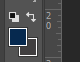
\includegraphics[width=0.9\textwidth]{images/foreground and background.png}
				\end{columns}
			\end{frame}
		

		\section{Manually Choosing Colors}
		\subsection{Color Panel}		
		\begin{frame}
			\frametitle{Color Panel}
			\begin{outline}
				\1 Panel in the top right corner.
				\1 Allows you to visually adjust the color and darkness.
			\end{outline}
			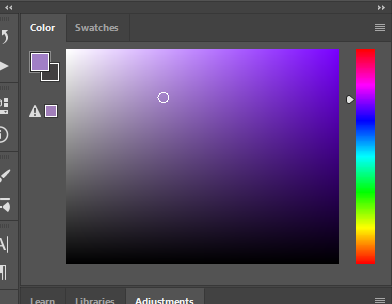
\includegraphics[width=0.7\textwidth]{images/color panel.png}
		\end{frame}
	
\subsection{Swatches Panel}		
\begin{frame}
	\frametitle{Swatches Panel}
	\begin{outline}
		\1 Panel in the top right corner.
		\1 Keeps track of the colours you have used.
		\1 Allows you to save colours and resuse them in the future.
	\end{outline}
	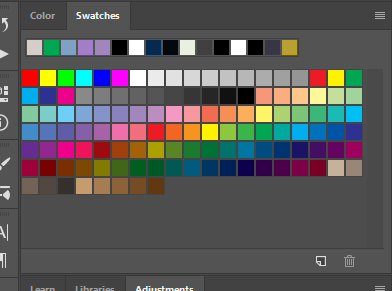
\includegraphics[width=0.7\textwidth]{images/swatches panel.png}
\end{frame}


	\section{Color Sampling Tools}
			\subsection{Eye Dropper Tool}		
	\begin{frame}
		\frametitle{Eye Dropper Tool}
			\begin{columns}
			\column{.6\textwidth}
			\vspace{-25pt}
				\begin{outline}
					\1 In the tools menu on the left-hand side.
					\1 Changes the foreground colour to whatever you click on.
					\1 The colour is also added to the swatches panel.
				\end{outline}
			\column{.45\textwidth}
				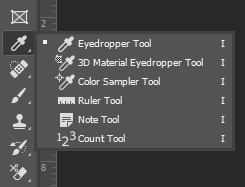
\includegraphics[width=1.0\textwidth]{images/Eye Dropper Tool.png}
			\end{columns}
		\end{frame}

			\subsection{Color Sampler Tool}		
				\begin{frame}
					\frametitle{Color Sampler Tool}
									\begin{outline}
						\1 Used to measure and view the color values in an image.
						\1 Stores the RBG values for each point you choose.
						\1 Points can be viewed in the Info panel.
					\end{outline}
					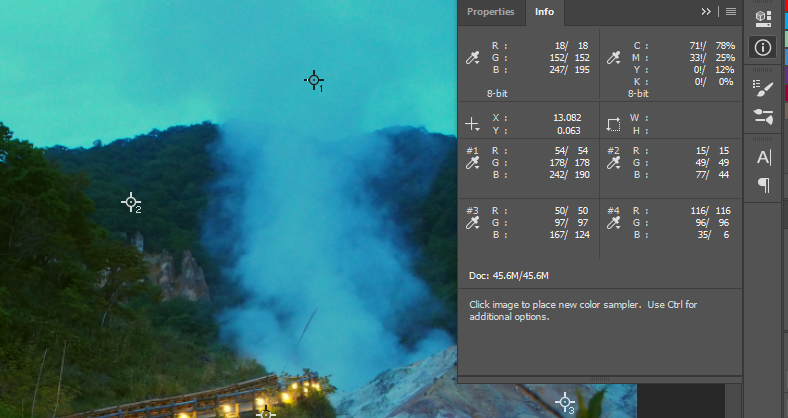
\includegraphics[width=0.85\textwidth]{images/color sampler tool.png}
				\end{frame}
			
					\section{Color Picker}
					\subsection{Color Picker}		
				\begin{frame}
					\frametitle{Color Picker}
														\begin{outline}
						\1 Double-click the Foreground color.  
						\1 This will open the Color Picker window.
						\1 Here you have everything in one place:
						\2 the Color panel
						\2 Eye dropper tool
						\2 Add to Swatches
						\2 RGB/CMYK values
						\2 Hex code 
					\end{outline}
				\begin{center}
					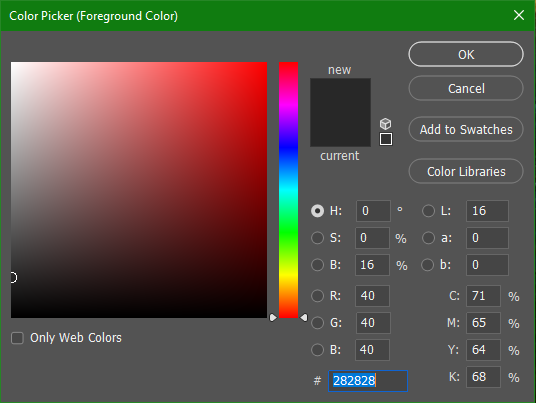
\includegraphics[width=0.45\textwidth]{images/color picker.png}
					\end{center}
				\end{frame}

	
\end{document}